\documentclass[11pt,a4paper]{article}
\usepackage[utf8x]{inputenc}
\usepackage[T1]{fontenc}
\usepackage{color}
\usepackage{multicol}
\usepackage{array}%création tableaux
\usepackage{graphicx}%pour les photosimages
\usepackage{subfigure}
% \usepackage{gentium}

\graphicspath{{figures}{../../resources-figures-jerboa}}

\usepackage{fancyhdr}
% \pagestyle{fancy}
% \renewcommand{\headrulewidth}{0pt}
% \renewcommand{\footrulewidth}{0pt}
% \setlength\headheight{80.0pt}
% \addtolength{\textheight}{-80.0pt}
% \chead{\includegraphics[scale=0.4]{Logo-template.PNG}}

\usepackage{mathptmx} % Use Times Font
\usepackage{geometry}
\geometry{
  a4paper,
  left=14mm,
  top=20mm,
  right =15mm,
  bottom =15mm
}
\pagestyle{fancy}
\renewcommand{\headrulewidth}{0pt}
\chead{\includegraphics[scale=1.2]{logos_corrig.pdf}}



\begin{document}

\begin{center}
  {\Large \textbf{Détection statique des changements topologiques dans le opérations de modélisation géométrique}}
\end{center}

\setlength\parindent{0em}%
\textbf{\underline{M. Gaide}$^{1}$, S. Jean$^{1}$, D. Marcheix$^{1}$, X. Skapin$^{2}$, A. Arnould$^{2}$, H. Belhaouari$^{2}$}%

\begin{flushright}
  \underline{Contact} : maxime.gaide@ensma.fr
\end{flushright}

\begin{flushleft}
  \scriptsize{
    $^1$, LIAS - IDD, ISAE-ENSMA\\%
    $^2$, XLIM - ASALI, Université de Poitiers%
  }
\end{flushleft}

\rule{1\linewidth}{3pt}

\setlength\parindent{0em} \normalsize{ \textbf{Mots-clés} : Modélisation
  géométrique à base topologique, Detection de modifications topologiques,
  Analyse statique, Règles de transformation de graphe, Cartes généralisée}

\vspace*{1em}

\normalsize{
  De nombreuses applications de modélisation géométrique nécessitent de détecter
  les changements topologiques effectués par les opérations de construction ou
  modification des objets, comme les scissions de faces ou les fusions de
  volumes par exemple. C'est pourquoi les API des noyaux de modeleurs permettent
  généralement d'accéder à ces informations. Ce suivi est effectué de manière
  dynamique en comparant les cellules topologiques (sommets, arrêtes, faces,
  volumes) avant et après chaque modification, ce qui est coûteux en temps de
  calcul.

  Dans cet exposé, nous proposons une méthode \emph{statique} pour détecter les
  changements topologiques. Pour cela nous utilisons une formalisation des
  modèles géométriques et de leurs opérations de manipulation : les cartes
  généralisées [1,2] et les transformations de graphes [3].
  Une analyse syntaxique des règles de transformation permet de calculer, de
  manière statique et avant toute application, les changements qui affecteront
  les entités topologiques. Nous définissons également de manière précise les
  cas limites dans lesquels il sera impossible d'affirmer qu'une entité
  topologique sera scindée ou fusionnée et où il sera donc nécessaire de
  procéder à une analyse dynamique ponctuelle du modèle. Une comparaison du coût
  des deux méthodes, dynamique et statique, de quelques opérations classiques
  sur les maillages permet de mesurer le gain.}%

\vspace*{1em}%

\begin{figure}[h!]
  \begin{minipage}[c]{.49\textwidth}
    \centering
    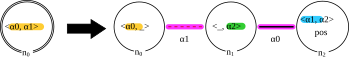
\includegraphics[width=\textwidth]{jdd-triangulation}%
    \caption{\footnotesize{\textbf{Règle de triangulation composée de deux
          membres. Son membre gauche, filtre une face et son membre droit la
          scinde.}}}
    \label{fig:rule-triangulation}
  \end{minipage}
  \hfill
  \begin{minipage}[c]{.24\textwidth}
    \centering
    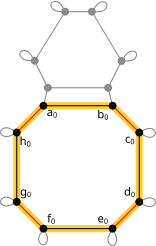
\includegraphics[height=.2\textheight]{jdd-triangulation-left}%
    \caption{\footnotesize{\textbf{Face incidente à $a_{0}$ (en orange), dans une G-carte.}}}
    \label{fig:tri-left}
  \end{minipage}
  \hfill
  \begin{minipage}[c]{.24\textwidth}
    \centering
    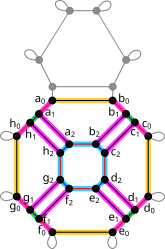
\includegraphics[height=.2\textheight]{jdd-triangulation-right}%
    \caption{\footnotesize{\textbf{Triangulation d'une face carrée.}}}
    \label{fig:tri-right}
  \end{minipage}
\end{figure}

\vspace*{1em}

\normalsize{% Par exemple, dans la règle de triangulation en
  % figure~\ref{fig:rule-triangulation}, son membre gauche, avec le nœud $n_{0}$,
  % filtre une face constituée de tous les brins atteignables par des liaisons
  % $\alpha 0$ (en noir) ou $\alpha 1$ (en rouge), exemple en
  % figure~\ref{fig:tri-left}. Dans son membre droit, la deuxième étiquettes de
  % tous les nœud est soit ``$\_$'' soit $\alpha 2$, autrement dit, il n'existe
  % plus de chemin uniquement composé de $\alpha 0$ et $\alpha 1$ entre toute
  % paire de brins de la face et celle-ci est scindée, exemple en
  % figure~\ref{fig:tri-right}.\\
  Cette méthode de détection statique est une première étape dans nos travaux
  pour la réévaluation de modèle. L'étape suivante portera sur son intégration
  dans le nommage persistant des entités topologiques pour, dans un premier
  temps, permettre le rejeu d'une séquence de règles, puis le rejeu d'une
  séquence d'opérations (ou scripts de règles).}

\begin{flushright}
  \rule{0.85\linewidth}{3pt}
\end{flushright}

\textbf{Références}

\footnotesize{$^{[1]}$ P.Lienhardt. Topological models for boundary
  representation: a comparison with n-dimensional generalized maps.
  Computer-aided design 23(1)(1991) 59-82.}

\footnotesize{$^{[2]}$ G.Damiand, P.Liendhardt. Combinatorial Maps: Efficient
  Data Structures for Computer Graphics and Image Processing. CRC Press(2014).}

\footnotesize{$^{[3]}$ H.Belhaouari, A.Arnould, P.Le Gall, T.Bellet. Jerboa: A
  graph transformation library for topology-based geometric modeling.
  International Conference on Graph Transformation(2014) 269-284.}

\end{document}
